\documentclass[12pt,a4paper]{article}

\usepackage[a4paper,text={16.5cm,25.2cm},centering]{geometry}
\usepackage{lmodern}
\usepackage{amssymb,amsmath}
\usepackage{bm}
\usepackage{graphicx}
\usepackage{microtype}
\usepackage{hyperref}
\setlength{\parindent}{0pt}
\setlength{\parskip}{1.2ex}

\hypersetup
       {   pdfauthor = { Marco Fasondini },
           pdftitle={ foo },
           colorlinks=TRUE,
           linkcolor=black,
           citecolor=blue,
           urlcolor=blue
       }




\usepackage{upquote}
\usepackage{listings}
\usepackage{xcolor}
\lstset{
    basicstyle=\ttfamily\footnotesize,
    upquote=true,
    breaklines=true,
    breakindent=0pt,
    keepspaces=true,
    showspaces=false,
    columns=fullflexible,
    showtabs=false,
    showstringspaces=false,
    escapeinside={(*@}{@*)},
    extendedchars=true,
}
\newcommand{\HLJLt}[1]{#1}
\newcommand{\HLJLw}[1]{#1}
\newcommand{\HLJLe}[1]{#1}
\newcommand{\HLJLeB}[1]{#1}
\newcommand{\HLJLo}[1]{#1}
\newcommand{\HLJLk}[1]{\textcolor[RGB]{148,91,176}{\textbf{#1}}}
\newcommand{\HLJLkc}[1]{\textcolor[RGB]{59,151,46}{\textit{#1}}}
\newcommand{\HLJLkd}[1]{\textcolor[RGB]{214,102,97}{\textit{#1}}}
\newcommand{\HLJLkn}[1]{\textcolor[RGB]{148,91,176}{\textbf{#1}}}
\newcommand{\HLJLkp}[1]{\textcolor[RGB]{148,91,176}{\textbf{#1}}}
\newcommand{\HLJLkr}[1]{\textcolor[RGB]{148,91,176}{\textbf{#1}}}
\newcommand{\HLJLkt}[1]{\textcolor[RGB]{148,91,176}{\textbf{#1}}}
\newcommand{\HLJLn}[1]{#1}
\newcommand{\HLJLna}[1]{#1}
\newcommand{\HLJLnb}[1]{#1}
\newcommand{\HLJLnbp}[1]{#1}
\newcommand{\HLJLnc}[1]{#1}
\newcommand{\HLJLncB}[1]{#1}
\newcommand{\HLJLnd}[1]{\textcolor[RGB]{214,102,97}{#1}}
\newcommand{\HLJLne}[1]{#1}
\newcommand{\HLJLneB}[1]{#1}
\newcommand{\HLJLnf}[1]{\textcolor[RGB]{66,102,213}{#1}}
\newcommand{\HLJLnfm}[1]{\textcolor[RGB]{66,102,213}{#1}}
\newcommand{\HLJLnp}[1]{#1}
\newcommand{\HLJLnl}[1]{#1}
\newcommand{\HLJLnn}[1]{#1}
\newcommand{\HLJLno}[1]{#1}
\newcommand{\HLJLnt}[1]{#1}
\newcommand{\HLJLnv}[1]{#1}
\newcommand{\HLJLnvc}[1]{#1}
\newcommand{\HLJLnvg}[1]{#1}
\newcommand{\HLJLnvi}[1]{#1}
\newcommand{\HLJLnvm}[1]{#1}
\newcommand{\HLJLl}[1]{#1}
\newcommand{\HLJLld}[1]{\textcolor[RGB]{148,91,176}{\textit{#1}}}
\newcommand{\HLJLs}[1]{\textcolor[RGB]{201,61,57}{#1}}
\newcommand{\HLJLsa}[1]{\textcolor[RGB]{201,61,57}{#1}}
\newcommand{\HLJLsb}[1]{\textcolor[RGB]{201,61,57}{#1}}
\newcommand{\HLJLsc}[1]{\textcolor[RGB]{201,61,57}{#1}}
\newcommand{\HLJLsd}[1]{\textcolor[RGB]{201,61,57}{#1}}
\newcommand{\HLJLsdB}[1]{\textcolor[RGB]{201,61,57}{#1}}
\newcommand{\HLJLsdC}[1]{\textcolor[RGB]{201,61,57}{#1}}
\newcommand{\HLJLse}[1]{\textcolor[RGB]{59,151,46}{#1}}
\newcommand{\HLJLsh}[1]{\textcolor[RGB]{201,61,57}{#1}}
\newcommand{\HLJLsi}[1]{#1}
\newcommand{\HLJLso}[1]{\textcolor[RGB]{201,61,57}{#1}}
\newcommand{\HLJLsr}[1]{\textcolor[RGB]{201,61,57}{#1}}
\newcommand{\HLJLss}[1]{\textcolor[RGB]{201,61,57}{#1}}
\newcommand{\HLJLssB}[1]{\textcolor[RGB]{201,61,57}{#1}}
\newcommand{\HLJLnB}[1]{\textcolor[RGB]{59,151,46}{#1}}
\newcommand{\HLJLnbB}[1]{\textcolor[RGB]{59,151,46}{#1}}
\newcommand{\HLJLnfB}[1]{\textcolor[RGB]{59,151,46}{#1}}
\newcommand{\HLJLnh}[1]{\textcolor[RGB]{59,151,46}{#1}}
\newcommand{\HLJLni}[1]{\textcolor[RGB]{59,151,46}{#1}}
\newcommand{\HLJLnil}[1]{\textcolor[RGB]{59,151,46}{#1}}
\newcommand{\HLJLnoB}[1]{\textcolor[RGB]{59,151,46}{#1}}
\newcommand{\HLJLoB}[1]{\textcolor[RGB]{102,102,102}{\textbf{#1}}}
\newcommand{\HLJLow}[1]{\textcolor[RGB]{102,102,102}{\textbf{#1}}}
\newcommand{\HLJLp}[1]{#1}
\newcommand{\HLJLc}[1]{\textcolor[RGB]{153,153,119}{\textit{#1}}}
\newcommand{\HLJLch}[1]{\textcolor[RGB]{153,153,119}{\textit{#1}}}
\newcommand{\HLJLcm}[1]{\textcolor[RGB]{153,153,119}{\textit{#1}}}
\newcommand{\HLJLcp}[1]{\textcolor[RGB]{153,153,119}{\textit{#1}}}
\newcommand{\HLJLcpB}[1]{\textcolor[RGB]{153,153,119}{\textit{#1}}}
\newcommand{\HLJLcs}[1]{\textcolor[RGB]{153,153,119}{\textit{#1}}}
\newcommand{\HLJLcsB}[1]{\textcolor[RGB]{153,153,119}{\textit{#1}}}
\newcommand{\HLJLg}[1]{#1}
\newcommand{\HLJLgd}[1]{#1}
\newcommand{\HLJLge}[1]{#1}
\newcommand{\HLJLgeB}[1]{#1}
\newcommand{\HLJLgh}[1]{#1}
\newcommand{\HLJLgi}[1]{#1}
\newcommand{\HLJLgo}[1]{#1}
\newcommand{\HLJLgp}[1]{#1}
\newcommand{\HLJLgs}[1]{#1}
\newcommand{\HLJLgsB}[1]{#1}
\newcommand{\HLJLgt}[1]{#1}



\def\qqand{\qquad\hbox{and}\qquad}
\def\qqfor{\qquad\hbox{for}\qquad}
\def\qqas{\qquad\hbox{as}\qquad}
\def\half{ {1 \over 2} }
\def\D{ {\rm d} }
\def\I{ {\rm i} }
\def\E{ {\rm e} }
\def\C{ {\mathbb C} }
\def\R{ {\mathbb R} }
\def\bbR{ {\mathbb R} }
\def\H{ {\mathbb H} }
\def\Z{ {\mathbb Z} }
\def\CC{ {\cal C} }
\def\FF{ {\cal F} }
\def\HH{ {\cal H} }
\def\LL{ {\cal L} }
\def\vc#1{ {\mathbf #1} }
\def\bbC{ {\mathbb C} }



\def\fR{ f_{\rm R} }
\def\fL{ f_{\rm L} }

\def\qqqquad{\qquad\qquad}
\def\qqwhere{\qquad\hbox{where}\qquad}
\def\Res_#1{\underset{#1}{\rm Res}\,}
\def\sech{ {\rm sech}\, }
\def\acos{ {\rm acos}\, }
\def\asin{ {\rm asin}\, }
\def\atan{ {\rm atan}\, }
\def\Ei{ {\rm Ei}\, }
\def\upepsilon{\varepsilon}


\def\Xint#1{ \mathchoice
   {\XXint\displaystyle\textstyle{#1} }%
   {\XXint\textstyle\scriptstyle{#1} }%
   {\XXint\scriptstyle\scriptscriptstyle{#1} }%
   {\XXint\scriptscriptstyle\scriptscriptstyle{#1} }%
   \!\int}
\def\XXint#1#2#3{ {\setbox0=\hbox{$#1{#2#3}{\int}$}
     \vcenter{\hbox{$#2#3$}}\kern-.5\wd0} }
\def\ddashint{\Xint=}
\def\dashint{\Xint-}
% \def\dashint
\def\infdashint{\dashint_{-\infty}^\infty}




\def\addtab#1={#1\;&=}
\def\ccr{\\\addtab}
\def\ip<#1>{\left\langle{#1}\right\rangle}
\def\dx{\D x}
\def\dt{\D t}
\def\dz{\D z}
\def\ds{\D s}

\def\rR{ {\rm R} }
\def\rL{ {\rm L} }

\def\norm#1{\left\| #1 \right\|}

\def\pr(#1){\left({#1}\right)}
\def\br[#1]{\left[{#1}\right]}

\def\abs#1{\left|{#1}\right|}
\def\fpr(#1){\!\pr({#1})}

\def\sopmatrix#1{ \begin{pmatrix}#1\end{pmatrix} }

\def\endash{–}
\def\emdash{—}
\def\mdblksquare{\blacksquare}
\def\lgblksquare{\blacksquare}
\def\scre{\E}
\def\mapengine#1,#2.{\mapfunction{#1}\ifx\void#2\else\mapengine #2.\fi }

\def\map[#1]{\mapengine #1,\void.}

\def\mapenginesep_#1#2,#3.{\mapfunction{#2}\ifx\void#3\else#1\mapengine #3.\fi }

\def\mapsep_#1[#2]{\mapenginesep_{#1}#2,\void.}


\def\vcbr[#1]{\pr(#1)}


\def\bvect[#1,#2]{
{
\def\dots{\cdots}
\def\mapfunction##1{\ | \  ##1}
	\sopmatrix{
		 \,#1\map[#2]\,
	}
}
}



\def\vect[#1]{
{\def\dots{\ldots}
	\vcbr[{#1}]
} }

\def\vectt[#1]{
{\def\dots{\ldots}
	\vect[{#1}]^{\top}
} }

\def\Vectt[#1]{
{
\def\mapfunction##1{##1 \cr}
\def\dots{\vdots}
	\begin{pmatrix}
		\map[#1]
	\end{pmatrix}
} }

\def\addtab#1={#1\;&=}
\def\ccr{\\\addtab}

\def\questionequals{= \!\!\!\!\!\!{\scriptstyle ? \atop }\,\,\,}

\def\Ei{\rm Ei\,}

\begin{document}

\section{Chapter 1: From finite differences to a spectral method for periodic functions}
Here we discuss

\begin{itemize}
\item[1. ] Finite difference (FD) approximations to the derivative of periodic functions


\item[2. ] How to construct FD formulas using interpolating polynomials


\item[3. ] How to analyse the accuracy of FD approximations using Taylor's theorem


\item[4. ] Differentiation matrices


\item[5. ] An example of exponentially fast convergence of a spectral method

\end{itemize}
\subsection{Finite difference approximations to the derivative}
Throughout this chapter, we consider a function $f(x)$ that is $2\pi$-periodic, i.e., $f(x+2\pi) = f(x)$ for $x \in \mathbb{R}$ and we suppose we have function values at equally spaced points on the interval $[0, 2\pi)$, i.e., we have $f(x_j)$, where

\[
x_j = jh, \qquad h = \frac{2\pi}{n}, \qquad j = 0, \ldots, n-1.
\]
How can we approximate $f'(x_j)$?

Recall that

\[
f'(x_j) = \lim_{\epsilon \to 0} \frac{f(x_j +\epsilon) - f(x_j)}{\epsilon},
\]
this suggests that for small $h$,

\[
f'(x_j) \approx \frac{f(x_j+h)-f(x_j)}{h} = \frac{f(x_{j+1})-f(x_j)}{h}. 
\]
This is an example of a \textbf{finite difference} approximation to a derivative of a function.  This particular approximation is known as a \emph{forward difference} approximation (or formula).  Replacing $h$ with $-h$, we obtain a \emph{backward difference} formula

\[
f'(x_j) \approx \frac{f(x_{j})-f(x_{j-1})}{h}.
\]
Finite difference formulae are used to design finite difference methods for PDEs, as we'll see later in this module.

Here is the \emph{central difference} formula

\[
f'(x_j) \approx \frac{f(x_{j+1})-f(x_{j-1})}{2h}.
\]
To analyse the accuracy of finite difference formulae, we recall Taylor's Theorem:

\textbf{Theorem (Taylor's Theorem)}  Let $a<b$, $n$ a positive integer, $x\in[a,b]$ and $f: [a,b]\to\mathbb{R}$ be a continuous function such that the derivatives up to order $n+1$ (inclusive) exist at every point in $[a,b]$. Then, for every $x\in[a,b]$, there exists a $\xi$ between $x$ and $x+h$ with $x+h\in[a,b]$, such that

\[
f(x+h)=\sum_{k=0}^{n}\frac{h^k}{k!}f^{(k)}(x)+\frac{h^{n+1}}{(n+1)!}f^{(n+1)}(\xi).
\]
\textbf{Corollary (central difference is 2nd order accurate)} Suppose $f \in C^3[x_{j-1},x_{j+1}]$ (i.e., the derivatives of orders $0, 1, 2, 3$ are continuous on $[x_{j-1},x_{j+1}]$), then 

\[
\left\vert\frac{f(x_{j+1})-f(x_{j-1})}{2h} - f'(x_j) \right\vert \leq \frac{M}{6}h^2, 
\]
where $M = \sup_{x \in [x_{j-1}, x_{j+1}]} \vert f'''(x) \vert$.

\textbf{Proof}

It follows from Taylor's theorem that there exists an $\xi_1 \in [x_{j}, x_{j+1}]$ such that 

\[
f(x_{j+ 1}) = f(x_{j + 1}) = f(x_j + h) = f(x_j) + h f'(x_j) + \frac{h^2}{2}f''(x_j) + \frac{h^3}{6}f'''(\xi_1).
\]
Similarly, there exists an $\xi_2 \in [x_{j-1}, x_{j}]$ such that 

\[
f(x_{j- 1}) = f(x_j) - h f'(x_j) + \frac{h}{2}f''(x_j) - \frac{h^3}{6}f'''(\xi_2).
\]
Therefore,

\[
\frac{f(x_{j+1})-f(x_{j-1})}{2h} = f'(x_j) + \frac{h^2}{12}\left( f'''(\xi_1) + f'''(\xi_2)   \right),
\]
from which the result follows. $\blacksquare$

Recalling the definition of big O notation, we can write

\[
f'(x_j) = \frac{f(x_{j+1})-f(x_{j-1})}{2h} + \mathcal{O}(h^2), \qquad h \to 0,
\]
and we say that the central difference approximation is second order accurate.  Similarly, we can show that the forward and backward difference approximations are first order approximations of the derivative.

\subsection{Finite differences via Lagrange interpolating polynomials}
How can we construct finite difference approximations?  One approach is via interpolating polynomials (aka polynomial interpolants or interpolatory polynomials).

\subsubsection{Interpolation}
\textbf{Definition (interpolation)}  We say that a function $p(x)$ interpolates a function $f(x)$ at the nodes / grid $x_{j}$, $j = 0, \ldots, n-1$ if 

\[
p(x_j) = f(x_j), \qquad j = 0, \ldots, n-1.
\]
The function values $f(x_j)$ are sometimes referred to as samples.

Here we use ApproxFun.jl (or Chebfun in Matlab) to construct an interpolant of a $2\pi$-periodic function.  In the next lecture we'll learn that this interpolant is not a polynomial in $x$ but rather it's a 'trigonometric interpolant' consisting of sines and cosines. (Later in this module, we'll learn more about the 'approximation technology' operating under the hood in ApproxFun and Chebfun.)


\begin{lstlisting}
(*@\HLJLk{using}@*) (*@\HLJLn{ApproxFun}@*)(*@\HLJLp{,}@*) (*@\HLJLn{Plots}@*)(*@\HLJLp{,}@*) (*@\HLJLn{LinearAlgebra}@*)(*@\HLJLp{,}@*) (*@\HLJLn{SparseArrays}@*)(*@\HLJLp{,}@*) (*@\HLJLn{ToeplitzMatrices}@*)
(*@\HLJLcs{{\#}}@*) (*@\HLJLcs{plot}@*) (*@\HLJLcs{a}@*) (*@\HLJLcs{2\ensuremath{\pi}-periodic}@*) (*@\HLJLcs{function}@*) (*@\HLJLcs{f}@*)
(*@\HLJLn{f}@*) (*@\HLJLoB{=}@*) (*@\HLJLnf{Fun}@*)(*@\HLJLp{(}@*)(*@\HLJLn{x}@*) (*@\HLJLoB{->}@*) (*@\HLJLni{1}@*)(*@\HLJLoB{/}@*)(*@\HLJLp{(}@*)(*@\HLJLnf{cos}@*)(*@\HLJLp{(}@*)(*@\HLJLn{x}@*)(*@\HLJLp{)}@*)(*@\HLJLoB{+}@*)(*@\HLJLni{2}@*)(*@\HLJLp{),}@*)(*@\HLJLnfB{0..2}@*)(*@\HLJLn{\ensuremath{\pi}}@*)(*@\HLJLp{)}@*)
(*@\HLJLnf{plot}@*)(*@\HLJLp{(}@*)(*@\HLJLn{f}@*)(*@\HLJLp{,}@*)(*@\HLJLn{lw}@*)(*@\HLJLoB{=}@*)(*@\HLJLni{3}@*)(*@\HLJLp{,}@*)(*@\HLJLn{label}@*)(*@\HLJLoB{=}@*)(*@\HLJLs{"{}f(x)"{}}@*)(*@\HLJLp{)}@*)
(*@\HLJLcs{{\#}}@*) (*@\HLJLcs{construct}@*) (*@\HLJLcs{an}@*) (*@\HLJLcs{interpolant}@*) (*@\HLJLcs{through}@*) (*@\HLJLcs{n}@*) (*@\HLJLcs{equally}@*) (*@\HLJLcs{spaced}@*) (*@\HLJLcs{points}@*) (*@\HLJLcs{and}@*) (*@\HLJLcs{plot}@*) (*@\HLJLcs{it}@*)
(*@\HLJLn{n}@*) (*@\HLJLoB{=}@*) (*@\HLJLni{5}@*)
(*@\HLJLn{p}@*) (*@\HLJLoB{=}@*) (*@\HLJLnf{Fun}@*)(*@\HLJLp{(}@*)(*@\HLJLn{f}@*)(*@\HLJLp{,}@*)(*@\HLJLnf{Fourier}@*)(*@\HLJLp{(}@*)(*@\HLJLnfB{0..2}@*)(*@\HLJLn{\ensuremath{\pi}}@*)(*@\HLJLp{),}@*)(*@\HLJLn{n}@*)(*@\HLJLp{)}@*) (*@\HLJLcs{{\#}}@*) (*@\HLJLcs{interpolant}@*)
(*@\HLJLnf{plot!}@*)(*@\HLJLp{(}@*)(*@\HLJLn{p}@*)(*@\HLJLp{,}@*)(*@\HLJLn{lw}@*)(*@\HLJLoB{=}@*)(*@\HLJLni{2}@*)(*@\HLJLp{,}@*)(*@\HLJLn{label}@*)(*@\HLJLoB{=}@*)(*@\HLJLs{"{}interpolant}@*) (*@\HLJLs{p(x)"{}}@*)(*@\HLJLp{)}@*)
(*@\HLJLcs{{\#}}@*) (*@\HLJLcs{show}@*) (*@\HLJLcs{the}@*) (*@\HLJLcs{interpolant}@*) (*@\HLJLcs{interpolates}@*) (*@\HLJLcs{f(x)}@*) (*@\HLJLcs{at}@*) (*@\HLJLcs{the}@*) (*@\HLJLcs{interpolation}@*) (*@\HLJLcs{nodes}@*)
(*@\HLJLn{h}@*) (*@\HLJLoB{=}@*) (*@\HLJLni{2}@*)(*@\HLJLn{\ensuremath{\pi}}@*)(*@\HLJLoB{/}@*)(*@\HLJLn{n}@*)(*@\HLJLp{;}@*)
(*@\HLJLn{xn}@*) (*@\HLJLoB{=}@*) (*@\HLJLni{0}@*)(*@\HLJLoB{:}@*)(*@\HLJLn{h}@*)(*@\HLJLoB{:}@*)(*@\HLJLni{2}@*)(*@\HLJLn{\ensuremath{\pi}}@*)(*@\HLJLoB{-}@*)(*@\HLJLn{h}@*) (*@\HLJLcs{{\#}}@*) (*@\HLJLcs{the}@*) (*@\HLJLcs{interpolation}@*) (*@\HLJLcs{nodes}@*)
(*@\HLJLnf{scatter!}@*)(*@\HLJLp{(}@*)(*@\HLJLn{xn}@*)(*@\HLJLp{,}@*)(*@\HLJLn{p}@*)(*@\HLJLoB{.}@*)(*@\HLJLp{(}@*)(*@\HLJLn{xn}@*)(*@\HLJLp{);}@*)(*@\HLJLn{label}@*)(*@\HLJLoB{=}@*)(*@\HLJLs{"{}f(x\ensuremath{\_j})}@*) (*@\HLJLs{=}@*) (*@\HLJLs{p(x\ensuremath{\_j})"{}}@*)(*@\HLJLp{)}@*)
\end{lstlisting}

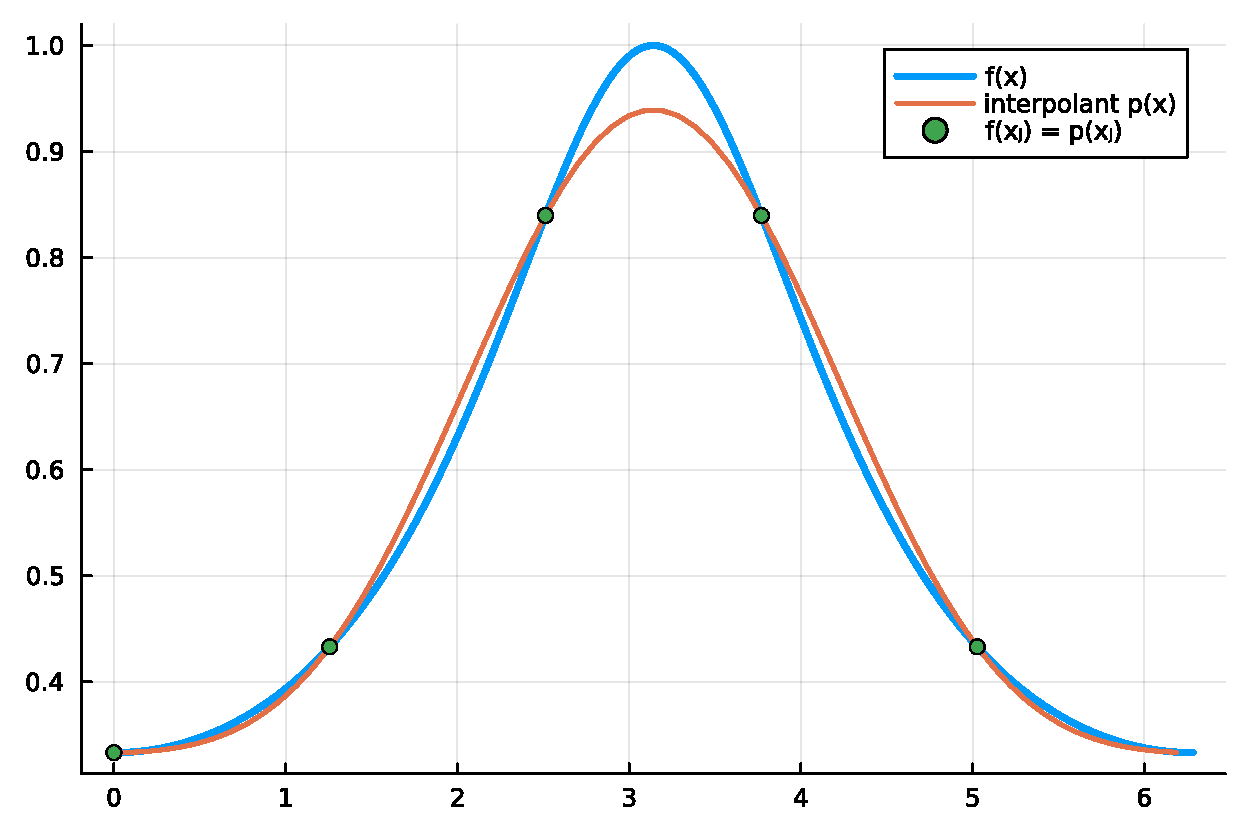
\includegraphics[width=\linewidth]{jl_6X9wr0/Ch1_FD_spectral_periodic_1_1.pdf}

A central idea in approximation methods is to approximate a function (which could be a solution to a differential equation, for example) with an interpolant, which are typically constructed from simple functions (e.g., polynomials, sines, cosines).  Hence, we approximate $f(x) \approx p(x)$ and here the idea is to  construct approximations to $f'(x)$ by differentiating $p(x)$, then we set $f'(x) \approx p'(x)$.

\subsubsection{Lagrange interpolation polynomials}
We can construct interpolatory polynomials directly. We will use the following polynomials which are equal to $1$ at one grid point and are zero at all the others:

\textbf{Definition (Lagrange basis polynomial)} The \emph{Lagrange basis polynomial} on the grid (or at the nodes)  $x_{j}$, $j = 0, \ldots, n-1$  is defined as

\[
\ensuremath{\ell}_k(x) := \prod_{\substack{j = 0 \\ j \neq k}}^{n-1} {x-x_j \over x_k - x_j} =  {(x-x_1) \ensuremath{\cdots}(x-x_{k-1})(x-x_{k+1}) \ensuremath{\cdots} (x-x_{n-1}) \over (x_k - x_1) \ensuremath{\cdots} (x_k - x_{k-1}) (x_k - x_{k+1}) \ensuremath{\cdots} (x_k - x_{n-1})}
\]
Plugging in the grid points verifies the following property:

\textbf{Proposition (delta interpolation)}

\[
\ensuremath{\ell}_k(x_j) = \ensuremath{\delta}_{kj} = \begin{cases}
1 & \text{if } j = k \\
0 & \text{if } j \neq k
\end{cases}
\]
We can use these to construct the interpolatory polynomial:

\textbf{Theorem (Lagrange interpolation)} The unique  polynomial of degree at most $n-1$ that interpolates $f$ at the $n$ distinct points $x_j$ is:

\[
p_n(x) = f(x_0) \ensuremath{\ell}_0(x) + \ensuremath{\cdots} + f(x_{n-1}) \ensuremath{\ell}_{n-1}(x)
\]
\textbf{Proof} Note that

\[
p_n(x_j) = \sum_{j=0}^{n-1} f(x_j) \ensuremath{\ell}_k(x_j) = f(x_j), \qquad j = 0, \ldots, n-1,
\]
and the fact that $p_n(x)$ is of degree $\leq n-1$ follows from the definition of the Lagrange basis polynomials, so we just need to show it is unique. Suppose $\tilde{p}_n(x)$ is a  polynomial of degree at most $n-1$ that also interpolates $f$. Then $\tilde{p}_n - p_n$ vanishes at $n$ distinct points. Thus by the fundamental theorem of algebra it must be zero.

\[
\blacksquare
\]
\textbf{Example} Construct the central difference approximation as follows: (i) construct the polynomial $p_3(x)$ that interpolates $f(x)$  at the three equally spaced points $x_{j-1}, x_j, x_{j+1}$; (ii) use $p_3(x)$ to approximate  $f'$ at $x_j$.

Using the formula for the Lagrange interpolating polynomial given above, it follows that (verify!)

\[
p_3(x) = \frac{(x-x_{j})(x-x_{j+1})}{2h^2}f(x_{j-1}) - \frac{(x-x_{j-1})(x-x_{j+1})}{h^2}f(x_{j}) + \frac{(x-x_{j-1})(x-x_{j})}{2h^2}f(x_{j+1})
\]
and

\[
p_3'(x_j) = \frac{f(x_{j+1}) - f(x_{j-1})}{2h}  \approx f'(x_j),
\]
which is the central difference approximation we've seen before.

\subsection{Differentiation matrices}
Collecting the approximations $p_3'(x_j) = \frac{f(x_{j+1}) - f(x_{j-1})}{2h}  \approx f'(x_j)$ for $j = 0, \ldots, n-1$ in a vector and using the fact that $f(x_{j+n}) = f(x_j + 2\pi) = f(x_{j})$, we obtain

\[
\left(
\begin{array}{c c c c c}
f'(x_0) \\
  \\
\vdots  \\
  \\
f'(x_{n-1})
\end{array}
\right) \approx 
\left(
\begin{array}{c c c c c}
p'(x_0) \\
  \\
\vdots  \\
  \\
p'(x_{n-1})
\end{array}
\right) = \frac{1}{h}
\left(
\begin{array}{c c c c c}
0 & \frac{1}{2} &   &   &  -\frac{1}{2} \\
-\frac{1}{2} & 0 & \ddots &  &  \\
   &   & \ddots &  &   \\
   &   & \ddots & 0 &  \frac{1}{2} \\
 \frac{1}{2}  &   &   & -\frac{1}{2} & 0
\end{array}
\right)
\left(
\begin{array}{c c c c c}
f(x_0) \\
  \\
\vdots  \\
  \\
f(x_{n-1})
\end{array}
\right).
\]
Note that omitted entries of the matrix are zero.  In vector notation, we can express this as

\[
\mathbf{f}' \approx \mathbf{p}' = D_n\mathbf{f}.
\]
The matrix $D_n$ is an example of a \textbf{differentiation matrix}; this differentiation matrix is skew-symmetric ($D_n^{\top} = -D_n$), Toeplitz (a matrix that is constant along its diagonals) and \href{https://en.wikipedia.org/wiki/Circulant_matrix}{circulant}.  

We can use the following command in Julia to create a sparse version of the differentiation matrix:


\begin{lstlisting}
(*@\HLJLn{n}@*) (*@\HLJLoB{=}@*) (*@\HLJLni{10}@*)
(*@\HLJLnf{spdiagm}@*)(*@\HLJLp{(}@*)(*@\HLJLni{1}@*)(*@\HLJLoB{=>}@*)(*@\HLJLnf{fill}@*)(*@\HLJLp{(}@*)(*@\HLJLnfB{0.5}@*)(*@\HLJLp{,}@*)(*@\HLJLn{n}@*)(*@\HLJLoB{-}@*)(*@\HLJLni{1}@*)(*@\HLJLp{),}@*)(*@\HLJLoB{-}@*)(*@\HLJLni{1}@*)(*@\HLJLoB{=>}@*)(*@\HLJLnf{fill}@*)(*@\HLJLp{(}@*)(*@\HLJLoB{-}@*)(*@\HLJLnfB{0.5}@*)(*@\HLJLp{,}@*)(*@\HLJLn{n}@*)(*@\HLJLoB{-}@*)(*@\HLJLni{1}@*)(*@\HLJLp{),}@*)(*@\HLJLn{n}@*)(*@\HLJLoB{-}@*)(*@\HLJLni{1}@*)(*@\HLJLoB{=>}@*)(*@\HLJLnf{fill}@*)(*@\HLJLp{(}@*)(*@\HLJLoB{-}@*)(*@\HLJLnfB{0.5}@*)(*@\HLJLp{,}@*)(*@\HLJLni{1}@*)(*@\HLJLp{),}@*)(*@\HLJLni{1}@*)(*@\HLJLoB{-}@*)(*@\HLJLn{n}@*)(*@\HLJLoB{=>}@*)(*@\HLJLnf{fill}@*)(*@\HLJLp{(}@*)(*@\HLJLnfB{0.5}@*)(*@\HLJLp{,}@*)(*@\HLJLni{1}@*)(*@\HLJLp{))}@*)
\end{lstlisting}

\begin{lstlisting}
10(*@\ensuremath{\times}@*)10 SparseArrays.SparseMatrixCSC(*@{{\{}}@*)Float64, Int64(*@{{\}}}@*) with 20 stored entries:
   (*@\ensuremath{\cdot}@*)    0.5    (*@\ensuremath{\cdot}@*)     (*@\ensuremath{\cdot}@*)     (*@\ensuremath{\cdot}@*)     (*@\ensuremath{\cdot}@*)     (*@\ensuremath{\cdot}@*)     (*@\ensuremath{\cdot}@*)     (*@\ensuremath{\cdot}@*)   -0.5
 -0.5    (*@\ensuremath{\cdot}@*)    0.5    (*@\ensuremath{\cdot}@*)     (*@\ensuremath{\cdot}@*)     (*@\ensuremath{\cdot}@*)     (*@\ensuremath{\cdot}@*)     (*@\ensuremath{\cdot}@*)     (*@\ensuremath{\cdot}@*)     (*@\ensuremath{\cdot}@*) 
   (*@\ensuremath{\cdot}@*)   -0.5    (*@\ensuremath{\cdot}@*)    0.5    (*@\ensuremath{\cdot}@*)     (*@\ensuremath{\cdot}@*)     (*@\ensuremath{\cdot}@*)     (*@\ensuremath{\cdot}@*)     (*@\ensuremath{\cdot}@*)     (*@\ensuremath{\cdot}@*) 
   (*@\ensuremath{\cdot}@*)     (*@\ensuremath{\cdot}@*)   -0.5    (*@\ensuremath{\cdot}@*)    0.5    (*@\ensuremath{\cdot}@*)     (*@\ensuremath{\cdot}@*)     (*@\ensuremath{\cdot}@*)     (*@\ensuremath{\cdot}@*)     (*@\ensuremath{\cdot}@*) 
   (*@\ensuremath{\cdot}@*)     (*@\ensuremath{\cdot}@*)     (*@\ensuremath{\cdot}@*)   -0.5    (*@\ensuremath{\cdot}@*)    0.5    (*@\ensuremath{\cdot}@*)     (*@\ensuremath{\cdot}@*)     (*@\ensuremath{\cdot}@*)     (*@\ensuremath{\cdot}@*) 
   (*@\ensuremath{\cdot}@*)     (*@\ensuremath{\cdot}@*)     (*@\ensuremath{\cdot}@*)     (*@\ensuremath{\cdot}@*)   -0.5    (*@\ensuremath{\cdot}@*)    0.5    (*@\ensuremath{\cdot}@*)     (*@\ensuremath{\cdot}@*)     (*@\ensuremath{\cdot}@*) 
   (*@\ensuremath{\cdot}@*)     (*@\ensuremath{\cdot}@*)     (*@\ensuremath{\cdot}@*)     (*@\ensuremath{\cdot}@*)     (*@\ensuremath{\cdot}@*)   -0.5    (*@\ensuremath{\cdot}@*)    0.5    (*@\ensuremath{\cdot}@*)     (*@\ensuremath{\cdot}@*) 
   (*@\ensuremath{\cdot}@*)     (*@\ensuremath{\cdot}@*)     (*@\ensuremath{\cdot}@*)     (*@\ensuremath{\cdot}@*)     (*@\ensuremath{\cdot}@*)     (*@\ensuremath{\cdot}@*)   -0.5    (*@\ensuremath{\cdot}@*)    0.5    (*@\ensuremath{\cdot}@*) 
   (*@\ensuremath{\cdot}@*)     (*@\ensuremath{\cdot}@*)     (*@\ensuremath{\cdot}@*)     (*@\ensuremath{\cdot}@*)     (*@\ensuremath{\cdot}@*)     (*@\ensuremath{\cdot}@*)     (*@\ensuremath{\cdot}@*)   -0.5    (*@\ensuremath{\cdot}@*)    0.5
  0.5    (*@\ensuremath{\cdot}@*)     (*@\ensuremath{\cdot}@*)     (*@\ensuremath{\cdot}@*)     (*@\ensuremath{\cdot}@*)     (*@\ensuremath{\cdot}@*)     (*@\ensuremath{\cdot}@*)     (*@\ensuremath{\cdot}@*)   -0.5    (*@\ensuremath{\cdot}@*)
\end{lstlisting}


For various values of $n$, let's compute the maximum error of the central difference approximation to the derivative at the points $x_j = jh$ with $j = 0, \ldots, n-1$ and $h = 2\pi/n$ for the function $f(x) = 1/(2 + \cos(x))$:


\begin{lstlisting}
(*@\HLJLn{f}@*) (*@\HLJLoB{=}@*) (*@\HLJLn{x}@*) (*@\HLJLoB{->}@*) (*@\HLJLni{1}@*)(*@\HLJLoB{/}@*)(*@\HLJLp{(}@*)(*@\HLJLni{2}@*) (*@\HLJLoB{+}@*) (*@\HLJLnf{cos}@*)(*@\HLJLp{(}@*)(*@\HLJLn{x}@*)(*@\HLJLp{))}@*)
(*@\HLJLn{Df}@*) (*@\HLJLoB{=}@*) (*@\HLJLn{x}@*) (*@\HLJLoB{->}@*) (*@\HLJLnf{sin}@*)(*@\HLJLp{(}@*)(*@\HLJLn{x}@*)(*@\HLJLp{)}@*)(*@\HLJLoB{/}@*)(*@\HLJLp{(}@*)(*@\HLJLni{2}@*) (*@\HLJLoB{+}@*) (*@\HLJLnf{cos}@*)(*@\HLJLp{(}@*)(*@\HLJLn{x}@*)(*@\HLJLp{))}@*)(*@\HLJLoB{{\textasciicircum}}@*)(*@\HLJLni{2}@*)  (*@\HLJLcs{{\#}}@*) (*@\HLJLcs{derivative}@*)
(*@\HLJLcs{{\#}}@*) (*@\HLJLcs{compute}@*) (*@\HLJLcs{the}@*) (*@\HLJLcs{errors}@*)
(*@\HLJLnd{@time}@*) (*@\HLJLk{begin}@*)
(*@\HLJLn{errs}@*) (*@\HLJLoB{=}@*) 
(*@\HLJLp{[(}@*) (*@\HLJLn{h}@*) (*@\HLJLoB{=}@*) (*@\HLJLni{2}@*)(*@\HLJLn{\ensuremath{\pi}}@*)(*@\HLJLoB{/}@*)(*@\HLJLn{n}@*)(*@\HLJLp{;}@*)
   (*@\HLJLcs{{\#}}@*) (*@\HLJLcs{differentiation}@*) (*@\HLJLcs{matrix:}@*)
   (*@\HLJLn{Dn}@*) (*@\HLJLoB{=}@*) (*@\HLJLni{1}@*)(*@\HLJLoB{/}@*)(*@\HLJLn{h}@*)(*@\HLJLoB{*}@*)(*@\HLJLnf{spdiagm}@*)(*@\HLJLp{(}@*)(*@\HLJLni{1}@*)(*@\HLJLoB{=>}@*)(*@\HLJLnf{fill}@*)(*@\HLJLp{(}@*)(*@\HLJLnfB{0.5}@*)(*@\HLJLp{,}@*)(*@\HLJLn{n}@*)(*@\HLJLoB{-}@*)(*@\HLJLni{1}@*)(*@\HLJLp{),}@*)(*@\HLJLoB{-}@*)(*@\HLJLni{1}@*)(*@\HLJLoB{=>}@*)(*@\HLJLnf{fill}@*)(*@\HLJLp{(}@*)(*@\HLJLoB{-}@*)(*@\HLJLnfB{0.5}@*)(*@\HLJLp{,}@*)(*@\HLJLn{n}@*)(*@\HLJLoB{-}@*)(*@\HLJLni{1}@*)(*@\HLJLp{),}@*)(*@\HLJLn{n}@*)(*@\HLJLoB{-}@*)(*@\HLJLni{1}@*)(*@\HLJLoB{=>}@*)(*@\HLJLnf{fill}@*)(*@\HLJLp{(}@*)(*@\HLJLoB{-}@*)(*@\HLJLnfB{0.5}@*)(*@\HLJLp{,}@*)(*@\HLJLni{1}@*)(*@\HLJLp{),}@*)(*@\HLJLni{1}@*)(*@\HLJLoB{-}@*)(*@\HLJLn{n}@*)(*@\HLJLoB{=>}@*)(*@\HLJLnf{fill}@*)(*@\HLJLp{(}@*)(*@\HLJLnfB{0.5}@*)(*@\HLJLp{,}@*)(*@\HLJLni{1}@*)(*@\HLJLp{));}@*)
   (*@\HLJLn{x}@*) (*@\HLJLoB{=}@*) (*@\HLJLnf{range}@*)(*@\HLJLp{(}@*)(*@\HLJLni{0}@*)(*@\HLJLp{,}@*)(*@\HLJLni{2}@*)(*@\HLJLn{\ensuremath{\pi}}@*)(*@\HLJLp{;}@*)(*@\HLJLn{length}@*)(*@\HLJLoB{=}@*)(*@\HLJLn{n}@*)(*@\HLJLoB{+}@*)(*@\HLJLni{1}@*)(*@\HLJLp{)[}@*)(*@\HLJLni{1}@*)(*@\HLJLoB{:}@*)(*@\HLJLk{end}@*)(*@\HLJLoB{-}@*)(*@\HLJLni{1}@*)(*@\HLJLp{];}@*) (*@\HLJLcs{{\#}}@*) (*@\HLJLcs{the}@*) (*@\HLJLcs{nodes}@*) (*@\HLJLcs{x\ensuremath{\_j},}@*) (*@\HLJLcs{j}@*) (*@\HLJLcs{=}@*) (*@\HLJLcs{0,}@*) (*@\HLJLcs{...,}@*) (*@\HLJLcs{n-1}@*)
   (*@\HLJLcs{{\#}}@*) (*@\HLJLcs{compute}@*) (*@\HLJLcs{the}@*) (*@\HLJLcs{maximum}@*) (*@\HLJLcs{error}@*) (*@\HLJLcs{at}@*) (*@\HLJLcs{the}@*) (*@\HLJLcs{nodes}@*)
   (*@\HLJLnf{norm}@*)(*@\HLJLp{(}@*)(*@\HLJLn{Dn}@*)(*@\HLJLoB{*}@*)(*@\HLJLn{f}@*)(*@\HLJLoB{.}@*)(*@\HLJLp{(}@*)(*@\HLJLn{x}@*)(*@\HLJLp{)}@*) (*@\HLJLoB{-}@*) (*@\HLJLn{Df}@*)(*@\HLJLoB{.}@*)(*@\HLJLp{(}@*)(*@\HLJLn{x}@*)(*@\HLJLp{),}@*)(*@\HLJLn{Inf}@*)(*@\HLJLp{)}@*) (*@\HLJLp{)}@*) (*@\HLJLk{for}@*) (*@\HLJLn{n}@*) (*@\HLJLoB{=}@*) (*@\HLJLn{Int64}@*)(*@\HLJLoB{.}@*)(*@\HLJLp{(}@*)(*@\HLJLn{round}@*)(*@\HLJLoB{.}@*)(*@\HLJLp{(}@*)(*@\HLJLni{10}@*) (*@\HLJLoB{.{\textasciicircum}}@*)(*@\HLJLp{(}@*)(*@\HLJLni{1}@*)(*@\HLJLoB{:}@*)(*@\HLJLnfB{0.5}@*)(*@\HLJLoB{:}@*)(*@\HLJLni{7}@*)(*@\HLJLp{)))]}@*)
(*@\HLJLk{end}@*)(*@\HLJLp{;}@*)
(*@\HLJLcs{{\#}}@*) (*@\HLJLcs{plot}@*) (*@\HLJLcs{the}@*) (*@\HLJLcs{errors}@*) (*@\HLJLcs{on}@*) (*@\HLJLcs{a}@*) (*@\HLJLcs{log-log}@*) (*@\HLJLcs{scale}@*)
(*@\HLJLn{D3f}@*) (*@\HLJLoB{=}@*) (*@\HLJLn{x}@*) (*@\HLJLoB{->}@*) (*@\HLJLp{(}@*)(*@\HLJLni{16}@*)(*@\HLJLoB{*}@*)(*@\HLJLnf{sin}@*)(*@\HLJLp{(}@*)(*@\HLJLni{2}@*)(*@\HLJLn{x}@*)(*@\HLJLp{)}@*) (*@\HLJLoB{+}@*) (*@\HLJLni{7}@*)(*@\HLJLoB{*}@*)(*@\HLJLnf{sin}@*)(*@\HLJLp{(}@*)(*@\HLJLn{x}@*)(*@\HLJLp{)}@*) (*@\HLJLoB{-}@*) (*@\HLJLnf{sin}@*)(*@\HLJLp{(}@*)(*@\HLJLni{3}@*)(*@\HLJLn{x}@*)(*@\HLJLp{))}@*)(*@\HLJLoB{/}@*)(*@\HLJLp{(}@*)(*@\HLJLni{4}@*)(*@\HLJLoB{*}@*)(*@\HLJLp{(}@*)(*@\HLJLni{2}@*) (*@\HLJLoB{+}@*) (*@\HLJLnf{cos}@*)(*@\HLJLp{(}@*)(*@\HLJLn{x}@*)(*@\HLJLp{))}@*)(*@\HLJLoB{{\textasciicircum}}@*)(*@\HLJLni{4}@*)(*@\HLJLp{)}@*) (*@\HLJLcs{{\#}}@*) (*@\HLJLcs{third}@*) (*@\HLJLcs{derivative}@*)
(*@\HLJLcs{{\#}}@*) (*@\HLJLcs{estimate}@*) (*@\HLJLcs{the}@*) (*@\HLJLcs{maximum}@*) (*@\HLJLcs{absolute}@*) (*@\HLJLcs{value}@*) (*@\HLJLcs{of}@*) (*@\HLJLcs{the}@*) (*@\HLJLcs{third}@*) (*@\HLJLcs{derivative}@*) (*@\HLJLcs{on}@*) (*@\HLJLcs{[-\ensuremath{\pi},}@*) (*@\HLJLcs{\ensuremath{\pi}]}@*)
(*@\HLJLn{xx}@*) (*@\HLJLoB{=}@*) (*@\HLJLnf{range}@*)(*@\HLJLp{(}@*)(*@\HLJLni{0}@*)(*@\HLJLp{,}@*)(*@\HLJLni{2}@*)(*@\HLJLn{\ensuremath{\pi}}@*)(*@\HLJLp{,}@*)(*@\HLJLni{1001}@*)(*@\HLJLp{)}@*)
(*@\HLJLn{M}@*) (*@\HLJLoB{=}@*) (*@\HLJLnf{norm}@*)(*@\HLJLp{(}@*)(*@\HLJLn{D3f}@*)(*@\HLJLoB{.}@*)(*@\HLJLp{(}@*)(*@\HLJLn{xx}@*)(*@\HLJLp{),}@*)(*@\HLJLn{Inf}@*)(*@\HLJLp{)}@*)
(*@\HLJLn{n}@*) (*@\HLJLoB{=}@*) (*@\HLJLni{10}@*) (*@\HLJLoB{.{\textasciicircum}}@*)(*@\HLJLp{(}@*)(*@\HLJLni{1}@*)(*@\HLJLoB{:}@*)(*@\HLJLnfB{0.5}@*)(*@\HLJLoB{:}@*)(*@\HLJLni{7}@*)(*@\HLJLp{)}@*)
(*@\HLJLnf{scatter}@*)(*@\HLJLp{(}@*)(*@\HLJLn{n}@*)(*@\HLJLp{,}@*)(*@\HLJLn{errs}@*)(*@\HLJLp{;}@*)(*@\HLJLn{xscale}@*)(*@\HLJLoB{=:}@*)(*@\HLJLn{log10}@*)(*@\HLJLp{,}@*)(*@\HLJLn{yscale}@*)(*@\HLJLoB{=:}@*)(*@\HLJLn{log10}@*)(*@\HLJLp{,}@*)(*@\HLJLn{label}@*)(*@\HLJLoB{=}@*)(*@\HLJLs{"{}Error"{}}@*)(*@\HLJLp{,}@*)(*@\HLJLn{xlabel}@*)(*@\HLJLoB{=}@*)(*@\HLJLs{"{}n"{}}@*)(*@\HLJLp{)}@*)
(*@\HLJLnf{plot!}@*)(*@\HLJLp{(}@*)(*@\HLJLn{n}@*)(*@\HLJLp{,}@*)(*@\HLJLn{M}@*)(*@\HLJLoB{*}@*)(*@\HLJLp{(}@*)(*@\HLJLni{2}@*)(*@\HLJLn{\ensuremath{\pi}}@*)(*@\HLJLp{)}@*)(*@\HLJLoB{{\textasciicircum}}@*)(*@\HLJLni{2}@*)(*@\HLJLoB{/}@*)(*@\HLJLni{6}@*)(*@\HLJLoB{*}@*)(*@\HLJLn{n}@*)(*@\HLJLoB{.{\textasciicircum}}@*)(*@\HLJLp{(}@*)(*@\HLJLoB{-}@*)(*@\HLJLni{2}@*)(*@\HLJLp{);}@*)(*@\HLJLn{label}@*)(*@\HLJLoB{=}@*)(*@\HLJLs{"{}upper}@*) (*@\HLJLs{bound}@*) (*@\HLJLs{on}@*) (*@\HLJLs{error"{}}@*)(*@\HLJLp{)}@*)
\end{lstlisting}

\begin{lstlisting}
4.506398 seconds (1.71 M allocations: 3.141 GiB, 21.40(*@{{\%}}@*) gc time, 22.36(*@{{\%}}@*) c
ompilation time)
\end{lstlisting}

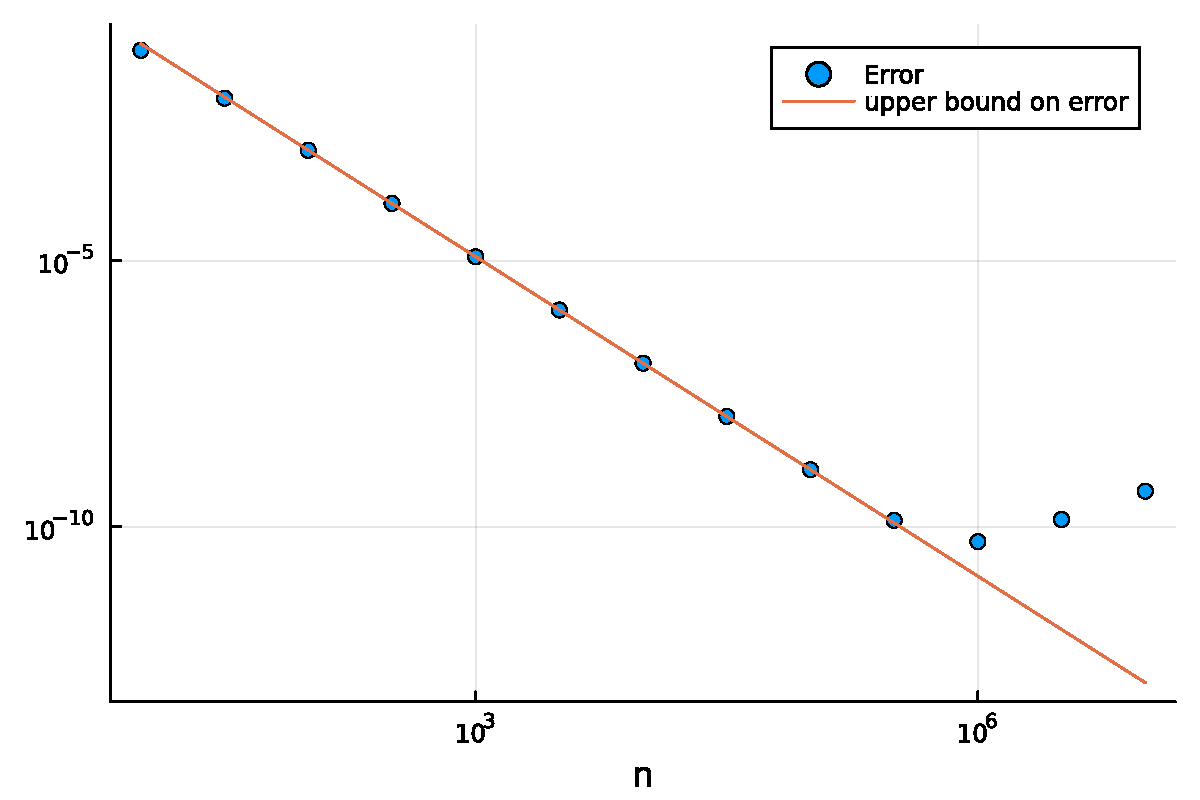
\includegraphics[width=\linewidth]{jl_6X9wr0/Ch1_FD_spectral_periodic_3_1.pdf}

\begin{lstlisting}
(*@\HLJLn{f}@*) (*@\HLJLoB{=}@*) (*@\HLJLn{x}@*) (*@\HLJLoB{->}@*) (*@\HLJLni{1}@*)(*@\HLJLoB{/}@*)(*@\HLJLp{(}@*)(*@\HLJLni{2}@*) (*@\HLJLoB{+}@*) (*@\HLJLnf{cos}@*)(*@\HLJLp{(}@*)(*@\HLJLn{x}@*)(*@\HLJLp{))}@*)
(*@\HLJLn{Df}@*) (*@\HLJLoB{=}@*) (*@\HLJLn{x}@*) (*@\HLJLoB{->}@*) (*@\HLJLnf{sin}@*)(*@\HLJLp{(}@*)(*@\HLJLn{x}@*)(*@\HLJLp{)}@*)(*@\HLJLoB{/}@*)(*@\HLJLp{(}@*)(*@\HLJLni{2}@*) (*@\HLJLoB{+}@*) (*@\HLJLnf{cos}@*)(*@\HLJLp{(}@*)(*@\HLJLn{x}@*)(*@\HLJLp{))}@*)(*@\HLJLoB{{\textasciicircum}}@*)(*@\HLJLni{2}@*)  (*@\HLJLcs{{\#}}@*) (*@\HLJLcs{derivative}@*)
(*@\HLJLcs{{\#}}@*) (*@\HLJLcs{compute}@*) (*@\HLJLcs{the}@*) (*@\HLJLcs{errors}@*)
(*@\HLJLn{nv}@*) (*@\HLJLoB{=}@*) (*@\HLJLn{Int64}@*)(*@\HLJLoB{.}@*)(*@\HLJLp{(}@*)(*@\HLJLn{round}@*)(*@\HLJLoB{.}@*)(*@\HLJLp{(}@*)(*@\HLJLni{10}@*) (*@\HLJLoB{.{\textasciicircum}}@*)(*@\HLJLp{(}@*)(*@\HLJLni{1}@*)(*@\HLJLoB{:}@*)(*@\HLJLnfB{0.5}@*)(*@\HLJLoB{:}@*)(*@\HLJLni{7}@*)(*@\HLJLp{)))}@*)
(*@\HLJLnd{@time}@*) (*@\HLJLk{begin}@*)
(*@\HLJLn{errs}@*) (*@\HLJLoB{=}@*) 
(*@\HLJLp{[(}@*) (*@\HLJLn{h}@*) (*@\HLJLoB{=}@*) (*@\HLJLni{2}@*)(*@\HLJLn{\ensuremath{\pi}}@*)(*@\HLJLoB{/}@*)(*@\HLJLn{n}@*)(*@\HLJLp{;}@*)
   (*@\HLJLcs{{\#}}@*) (*@\HLJLcs{differentiation}@*) (*@\HLJLcs{matrix:}@*)
   (*@\HLJLn{Dn}@*) (*@\HLJLoB{=}@*) (*@\HLJLni{1}@*)(*@\HLJLoB{/}@*)(*@\HLJLn{h}@*)(*@\HLJLoB{*}@*)(*@\HLJLnf{spdiagm}@*)(*@\HLJLp{(}@*)(*@\HLJLni{1}@*)(*@\HLJLoB{=>}@*)(*@\HLJLnf{fill}@*)(*@\HLJLp{(}@*)(*@\HLJLnfB{0.5}@*)(*@\HLJLp{,}@*)(*@\HLJLn{n}@*)(*@\HLJLoB{-}@*)(*@\HLJLni{1}@*)(*@\HLJLp{),}@*)(*@\HLJLoB{-}@*)(*@\HLJLni{1}@*)(*@\HLJLoB{=>}@*)(*@\HLJLnf{fill}@*)(*@\HLJLp{(}@*)(*@\HLJLoB{-}@*)(*@\HLJLnfB{0.5}@*)(*@\HLJLp{,}@*)(*@\HLJLn{n}@*)(*@\HLJLoB{-}@*)(*@\HLJLni{1}@*)(*@\HLJLp{),}@*)(*@\HLJLn{n}@*)(*@\HLJLoB{-}@*)(*@\HLJLni{1}@*)(*@\HLJLoB{=>}@*)(*@\HLJLnf{fill}@*)(*@\HLJLp{(}@*)(*@\HLJLoB{-}@*)(*@\HLJLnfB{0.5}@*)(*@\HLJLp{,}@*)(*@\HLJLni{1}@*)(*@\HLJLp{),}@*)(*@\HLJLni{1}@*)(*@\HLJLoB{-}@*)(*@\HLJLn{n}@*)(*@\HLJLoB{=>}@*)(*@\HLJLnf{fill}@*)(*@\HLJLp{(}@*)(*@\HLJLnfB{0.5}@*)(*@\HLJLp{,}@*)(*@\HLJLni{1}@*)(*@\HLJLp{));}@*)
   (*@\HLJLn{x}@*) (*@\HLJLoB{=}@*) (*@\HLJLnf{range}@*)(*@\HLJLp{(}@*)(*@\HLJLni{0}@*)(*@\HLJLp{,}@*)(*@\HLJLni{2}@*)(*@\HLJLn{\ensuremath{\pi}}@*)(*@\HLJLp{;}@*)(*@\HLJLn{length}@*)(*@\HLJLoB{=}@*)(*@\HLJLn{n}@*)(*@\HLJLoB{+}@*)(*@\HLJLni{1}@*)(*@\HLJLp{)[}@*)(*@\HLJLni{1}@*)(*@\HLJLoB{:}@*)(*@\HLJLk{end}@*)(*@\HLJLoB{-}@*)(*@\HLJLni{1}@*)(*@\HLJLp{];}@*) (*@\HLJLcs{{\#}}@*) (*@\HLJLcs{the}@*) (*@\HLJLcs{nodes}@*) (*@\HLJLcs{x\ensuremath{\_j},}@*) (*@\HLJLcs{j}@*) (*@\HLJLcs{=}@*) (*@\HLJLcs{0,}@*) (*@\HLJLcs{...,}@*) (*@\HLJLcs{n-1}@*)
   (*@\HLJLcs{{\#}}@*) (*@\HLJLcs{compute}@*) (*@\HLJLcs{the}@*) (*@\HLJLcs{maximum}@*) (*@\HLJLcs{error}@*) (*@\HLJLcs{at}@*) (*@\HLJLcs{the}@*) (*@\HLJLcs{nodes}@*)
   (*@\HLJLnf{norm}@*)(*@\HLJLp{(}@*)(*@\HLJLn{Dn}@*)(*@\HLJLoB{*}@*)(*@\HLJLn{f}@*)(*@\HLJLoB{.}@*)(*@\HLJLp{(}@*)(*@\HLJLn{x}@*)(*@\HLJLp{)}@*) (*@\HLJLoB{-}@*) (*@\HLJLn{Df}@*)(*@\HLJLoB{.}@*)(*@\HLJLp{(}@*)(*@\HLJLn{x}@*)(*@\HLJLp{),}@*)(*@\HLJLn{Inf}@*)(*@\HLJLp{)}@*) (*@\HLJLp{)}@*) (*@\HLJLk{for}@*) (*@\HLJLn{n}@*) (*@\HLJLoB{=}@*) (*@\HLJLn{nv}@*)(*@\HLJLp{]}@*)
(*@\HLJLk{end}@*)(*@\HLJLp{;}@*)
(*@\HLJLcs{{\#}}@*) (*@\HLJLcs{plot}@*) (*@\HLJLcs{the}@*) (*@\HLJLcs{errors}@*) (*@\HLJLcs{on}@*) (*@\HLJLcs{a}@*) (*@\HLJLcs{log-log}@*) (*@\HLJLcs{scale}@*)
(*@\HLJLn{D3f}@*) (*@\HLJLoB{=}@*) (*@\HLJLn{x}@*) (*@\HLJLoB{->}@*) (*@\HLJLp{(}@*)(*@\HLJLni{16}@*)(*@\HLJLoB{*}@*)(*@\HLJLnf{sin}@*)(*@\HLJLp{(}@*)(*@\HLJLni{2}@*)(*@\HLJLn{x}@*)(*@\HLJLp{)}@*) (*@\HLJLoB{+}@*) (*@\HLJLni{7}@*)(*@\HLJLoB{*}@*)(*@\HLJLnf{sin}@*)(*@\HLJLp{(}@*)(*@\HLJLn{x}@*)(*@\HLJLp{)}@*) (*@\HLJLoB{-}@*) (*@\HLJLnf{sin}@*)(*@\HLJLp{(}@*)(*@\HLJLni{3}@*)(*@\HLJLn{x}@*)(*@\HLJLp{))}@*)(*@\HLJLoB{/}@*)(*@\HLJLp{(}@*)(*@\HLJLni{4}@*)(*@\HLJLoB{*}@*)(*@\HLJLp{(}@*)(*@\HLJLni{2}@*) (*@\HLJLoB{+}@*) (*@\HLJLnf{cos}@*)(*@\HLJLp{(}@*)(*@\HLJLn{x}@*)(*@\HLJLp{))}@*)(*@\HLJLoB{{\textasciicircum}}@*)(*@\HLJLni{4}@*)(*@\HLJLp{)}@*) (*@\HLJLcs{{\#}}@*) (*@\HLJLcs{third}@*) (*@\HLJLcs{derivative}@*)
(*@\HLJLcs{{\#}}@*) (*@\HLJLcs{estimate}@*) (*@\HLJLcs{the}@*) (*@\HLJLcs{maximum}@*) (*@\HLJLcs{absolute}@*) (*@\HLJLcs{value}@*) (*@\HLJLcs{of}@*) (*@\HLJLcs{the}@*) (*@\HLJLcs{third}@*) (*@\HLJLcs{derivative}@*) (*@\HLJLcs{on}@*) (*@\HLJLcs{[-\ensuremath{\pi},}@*) (*@\HLJLcs{\ensuremath{\pi}]}@*)
(*@\HLJLn{xx}@*) (*@\HLJLoB{=}@*) (*@\HLJLnf{range}@*)(*@\HLJLp{(}@*)(*@\HLJLni{0}@*)(*@\HLJLp{,}@*)(*@\HLJLni{2}@*)(*@\HLJLn{\ensuremath{\pi}}@*)(*@\HLJLp{,}@*)(*@\HLJLni{1001}@*)(*@\HLJLp{)}@*)
(*@\HLJLn{M}@*) (*@\HLJLoB{=}@*) (*@\HLJLnf{norm}@*)(*@\HLJLp{(}@*)(*@\HLJLn{D3f}@*)(*@\HLJLoB{.}@*)(*@\HLJLp{(}@*)(*@\HLJLn{xx}@*)(*@\HLJLp{),}@*)(*@\HLJLn{Inf}@*)(*@\HLJLp{)}@*)
(*@\HLJLnf{scatter}@*)(*@\HLJLp{(}@*)(*@\HLJLn{nv}@*)(*@\HLJLp{,}@*)(*@\HLJLn{errs}@*)(*@\HLJLp{;}@*)(*@\HLJLn{xscale}@*)(*@\HLJLoB{=:}@*)(*@\HLJLn{log10}@*)(*@\HLJLp{,}@*)(*@\HLJLn{yscale}@*)(*@\HLJLoB{=:}@*)(*@\HLJLn{log10}@*)(*@\HLJLp{,}@*)(*@\HLJLn{label}@*)(*@\HLJLoB{=}@*)(*@\HLJLs{"{}Error"{}}@*)(*@\HLJLp{,}@*)(*@\HLJLn{xlabel}@*)(*@\HLJLoB{=}@*)(*@\HLJLs{"{}n"{}}@*)(*@\HLJLp{)}@*)
(*@\HLJLnf{plot!}@*)(*@\HLJLp{(}@*)(*@\HLJLn{nv}@*)(*@\HLJLp{,}@*)(*@\HLJLn{M}@*)(*@\HLJLoB{*}@*)(*@\HLJLp{(}@*)(*@\HLJLni{2}@*)(*@\HLJLn{\ensuremath{\pi}}@*)(*@\HLJLp{)}@*)(*@\HLJLoB{{\textasciicircum}}@*)(*@\HLJLni{2}@*)(*@\HLJLoB{/}@*)(*@\HLJLni{6}@*)(*@\HLJLoB{*}@*)(*@\HLJLn{nv}@*)(*@\HLJLoB{.{\textasciicircum}}@*)(*@\HLJLp{(}@*)(*@\HLJLoB{-}@*)(*@\HLJLni{2}@*)(*@\HLJLp{);}@*)(*@\HLJLn{label}@*)(*@\HLJLoB{=}@*)(*@\HLJLs{"{}upper}@*) (*@\HLJLs{bound}@*) (*@\HLJLs{on}@*) (*@\HLJLs{error"{}}@*)(*@\HLJLp{)}@*)
\end{lstlisting}

\begin{lstlisting}
3.493785 seconds (490.76 k allocations: 3.078 GiB, 17.46(*@{{\%}}@*) gc time, 7.94(*@{{\%}}@*) 
compilation time)
\end{lstlisting}

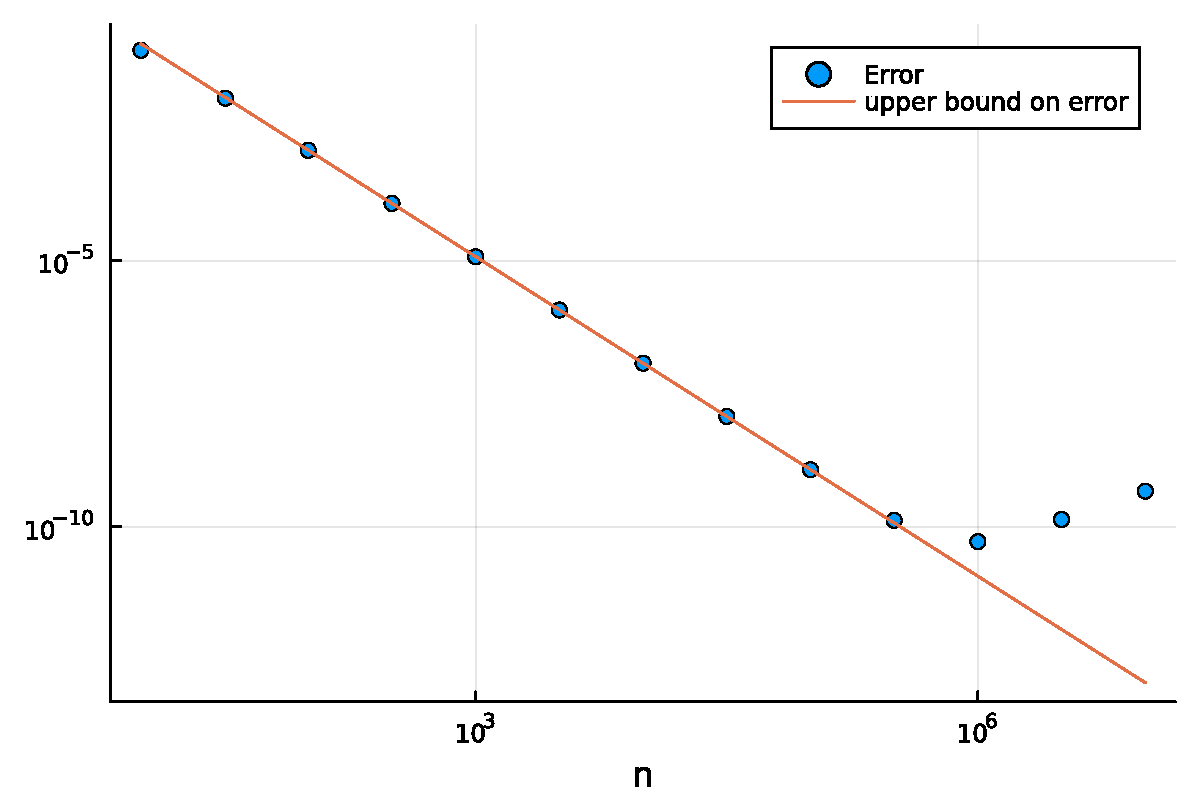
\includegraphics[width=\linewidth]{jl_6X9wr0/Ch1_FD_spectral_periodic_4_1.pdf}

The plot shows that the error decays as $\mathcal{O}(n^{-2})$, $n \to \infty$.

To derive a higher order finite difference approximation to the derivative, we can use a higher degree interpolating polynomial.  For example, let $m$ be even, then we can derive an $m$-th order central difference approximation to the derivative by 

\begin{itemize}
\item[1. ] constructing an interpolating polynomial $p_{m+1}(x)$ such that $p_{m+1}$ interpolates $f$ at $x_j$, $x_{j\pm 1}$, $x_{j\pm 2}$, $\ldots$,  $x_{j\pm m/2}$ and 


\item[2. ] making the approximation $f'(x_j) \approx p_{m+1}'(x_j)$. 

\end{itemize}
We have already carried out this procedure for $m = 2$. If we take $m = 4$, then we would obtain the following fourth-order central difference approximation to the derivative:

\[
f'(x_j) \approx p_5'(x_j) = \frac{f(x_{j-2}) -8 f(x_{j-1}) + 8 f(x_{j+1}) - f(x_{j-2})}{12h},
\]
whose error behaves as $\mathcal{O}(h^4)$, $h \to 0$ (or, equivalently, as $\mathcal{O}(n^{-4})$, $n \to \infty$) if $f$ is sufficiently smooth (e.g., if $f \in C^5[x_{j-2}, x_{j+2}]$).

What would the central difference approximation to the derivative be if we let $m \to \infty$? We won't prove this (see \emph{A Practical Guide to Pseudospectral Methods} by B. Fornberg if you're interested in the details) but using the fact that $f$ is $2\pi$-periodic, it can be shown that the central difference approximation obtained by letting $m \to \infty$ is equivalent to applying the following $n \times n$ differentiation matrix

\[
\left(
\begin{array}{c}
f'(x_0) \\
  \\
\vdots  \\
  \\
f'(x_{n-1})
\end{array}
\right) \approx 
\left(
\begin{array}{c}
p'(x_0) \\
  \\
\vdots  \\
  \\
p'(x_{n-1})
\end{array}
\right) = \frac{1}{h}
\left(
\begin{array}{c c c c c c c}
  &       &       & \vdots  &   &   & \\
  &\ddots &       & \frac{1}{2}\csc \frac{3h}{2}   &   &    &  \\
   &\ddots &      &-\frac{1}{2}\csc \frac{2h}{2}   &   &    &  \\ 
   &\ddots &      & \frac{1}{2}\csc \frac{1h}{2}   &   &    &   \\
  &        &      & 0                              &   &    &   \\
&      &      & -\frac{1}{2}\csc \frac{1h}{2}   &   &   \ddots &  \\
&      &      & \frac{1}{2}\csc \frac{2h}{2}   &   &   \ddots &  \\
&      &      & -\frac{1}{2}\csc \frac{3h}{2}   &   &   \ddots &  \\
&      &      & \ensuremath{\vdots}  &   &    &  
\end{array}
\right)
\left(
\begin{array}{c}
f(x_0) \\
  \\
\vdots  \\
  \\
f(x_{n-1})
\end{array}
\right).
\]
where $h = 2\pi/n$.  In the next chapter we shall derive this differentiation matrix via trigonometric interpolants.   Since this differentiation matrix is derived by letting $m \to \infty$, we expect the error to decay faster than $\mathcal{O}(n^{-m})$ for all $m > 0$, provided $f \in C^{\infty}[0, 2\pi]$.  Let's check this numerically:


\begin{lstlisting}
(*@\HLJLn{Nv}@*) (*@\HLJLoB{=}@*) (*@\HLJLni{5}@*)(*@\HLJLoB{:}@*)(*@\HLJLni{2}@*)(*@\HLJLoB{:}@*)(*@\HLJLni{71}@*)(*@\HLJLp{;}@*)
(*@\HLJLn{errs}@*) (*@\HLJLoB{=}@*) 
(*@\HLJLp{[(}@*) (*@\HLJLn{h}@*) (*@\HLJLoB{=}@*) (*@\HLJLni{2}@*)(*@\HLJLn{\ensuremath{\pi}}@*)(*@\HLJLoB{/}@*)(*@\HLJLn{N}@*)(*@\HLJLp{;}@*)
    (*@\HLJLn{column}@*) (*@\HLJLoB{=}@*) (*@\HLJLp{[}@*)(*@\HLJLni{0}@*)(*@\HLJLp{;}@*) (*@\HLJLnfB{0.5}@*)(*@\HLJLoB{*}@*)(*@\HLJLp{(}@*)(*@\HLJLoB{-}@*)(*@\HLJLni{1}@*)(*@\HLJLp{)}@*)(*@\HLJLoB{.{\textasciicircum}}@*)(*@\HLJLp{(}@*)(*@\HLJLni{1}@*)(*@\HLJLoB{:}@*)(*@\HLJLn{N}@*)(*@\HLJLoB{-}@*)(*@\HLJLni{1}@*)(*@\HLJLp{)}@*)(*@\HLJLoB{.*}@*)(*@\HLJLn{csc}@*)(*@\HLJLoB{.}@*)(*@\HLJLp{((}@*)(*@\HLJLni{1}@*)(*@\HLJLoB{:}@*)(*@\HLJLn{N}@*)(*@\HLJLoB{-}@*)(*@\HLJLni{1}@*)(*@\HLJLp{)}@*)(*@\HLJLoB{*}@*)(*@\HLJLn{h}@*)(*@\HLJLoB{/}@*)(*@\HLJLni{2}@*)(*@\HLJLp{)];}@*)
    (*@\HLJLcs{{\#}}@*) (*@\HLJLcs{Differentiation}@*) (*@\HLJLcs{matrix:}@*)
    (*@\HLJLn{D\ensuremath{\_m}}@*) (*@\HLJLoB{=}@*) (*@\HLJLnf{Toeplitz}@*)(*@\HLJLp{(}@*)(*@\HLJLn{column}@*)(*@\HLJLp{,[}@*)(*@\HLJLn{column}@*)(*@\HLJLp{[}@*)(*@\HLJLni{1}@*)(*@\HLJLp{];}@*) (*@\HLJLn{column}@*)(*@\HLJLp{[}@*)(*@\HLJLn{N}@*)(*@\HLJLoB{:-}@*)(*@\HLJLni{1}@*)(*@\HLJLoB{:}@*)(*@\HLJLni{2}@*)(*@\HLJLp{]]);}@*)
    (*@\HLJLcs{{\#}}@*) (*@\HLJLcs{N}@*) (*@\HLJLcs{equally}@*) (*@\HLJLcs{spaced}@*) (*@\HLJLcs{points}@*) (*@\HLJLcs{on}@*) (*@\HLJLcs{[-\ensuremath{\pi},}@*) (*@\HLJLcs{\ensuremath{\pi})}@*)
    (*@\HLJLn{x}@*) (*@\HLJLoB{=}@*) (*@\HLJLnf{range}@*)(*@\HLJLp{(}@*)(*@\HLJLni{0}@*)(*@\HLJLp{,}@*)(*@\HLJLni{2}@*)(*@\HLJLn{\ensuremath{\pi}}@*)(*@\HLJLp{;}@*)(*@\HLJLn{length}@*)(*@\HLJLoB{=}@*)(*@\HLJLn{N}@*)(*@\HLJLoB{+}@*)(*@\HLJLni{1}@*)(*@\HLJLp{)[}@*)(*@\HLJLni{1}@*)(*@\HLJLoB{:}@*)(*@\HLJLk{end}@*)(*@\HLJLoB{-}@*)(*@\HLJLni{1}@*)(*@\HLJLp{];}@*)
    (*@\HLJLcs{{\#}}@*) (*@\HLJLcs{maximum}@*) (*@\HLJLcs{error}@*) (*@\HLJLcs{at}@*) (*@\HLJLcs{the}@*) (*@\HLJLcs{set}@*) (*@\HLJLcs{of}@*) (*@\HLJLcs{N}@*) (*@\HLJLcs{points}@*)
    (*@\HLJLnf{norm}@*)(*@\HLJLp{(}@*)(*@\HLJLn{D\ensuremath{\_m}}@*)(*@\HLJLoB{*}@*)(*@\HLJLn{f}@*)(*@\HLJLoB{.}@*)(*@\HLJLp{(}@*)(*@\HLJLn{x}@*)(*@\HLJLp{)}@*) (*@\HLJLoB{-}@*) (*@\HLJLn{Df}@*)(*@\HLJLoB{.}@*)(*@\HLJLp{(}@*)(*@\HLJLn{x}@*)(*@\HLJLp{),}@*)(*@\HLJLn{Inf}@*)(*@\HLJLp{)}@*) (*@\HLJLp{)}@*) (*@\HLJLk{for}@*) (*@\HLJLn{N}@*) (*@\HLJLoB{=}@*) (*@\HLJLn{Nv}@*)(*@\HLJLp{]}@*)
(*@\HLJLcs{{\#}}@*) (*@\HLJLcs{plot}@*) (*@\HLJLcs{the}@*) (*@\HLJLcs{error}@*) (*@\HLJLcs{on}@*) (*@\HLJLcs{a}@*) (*@\HLJLcs{semi-log}@*) (*@\HLJLcs{(log-linear)}@*) (*@\HLJLcs{scale}@*)
(*@\HLJLnf{scatter}@*)(*@\HLJLp{(}@*)(*@\HLJLn{Nv}@*)(*@\HLJLp{,}@*)(*@\HLJLn{errs}@*)(*@\HLJLp{;}@*)(*@\HLJLn{yscale}@*)(*@\HLJLoB{=:}@*)(*@\HLJLn{log10}@*)(*@\HLJLp{,}@*)(*@\HLJLn{label}@*)(*@\HLJLoB{=}@*)(*@\HLJLs{"{}Error"{}}@*)(*@\HLJLp{)}@*)
(*@\HLJLnf{plot!}@*)(*@\HLJLp{(}@*)(*@\HLJLn{Nv}@*)(*@\HLJLp{,(}@*)(*@\HLJLnfB{1.85}@*)(*@\HLJLp{)}@*)(*@\HLJLoB{.{\textasciicircum}}@*)(*@\HLJLp{(}@*)(*@\HLJLoB{-}@*)(*@\HLJLn{Nv}@*)(*@\HLJLp{))}@*)
\end{lstlisting}

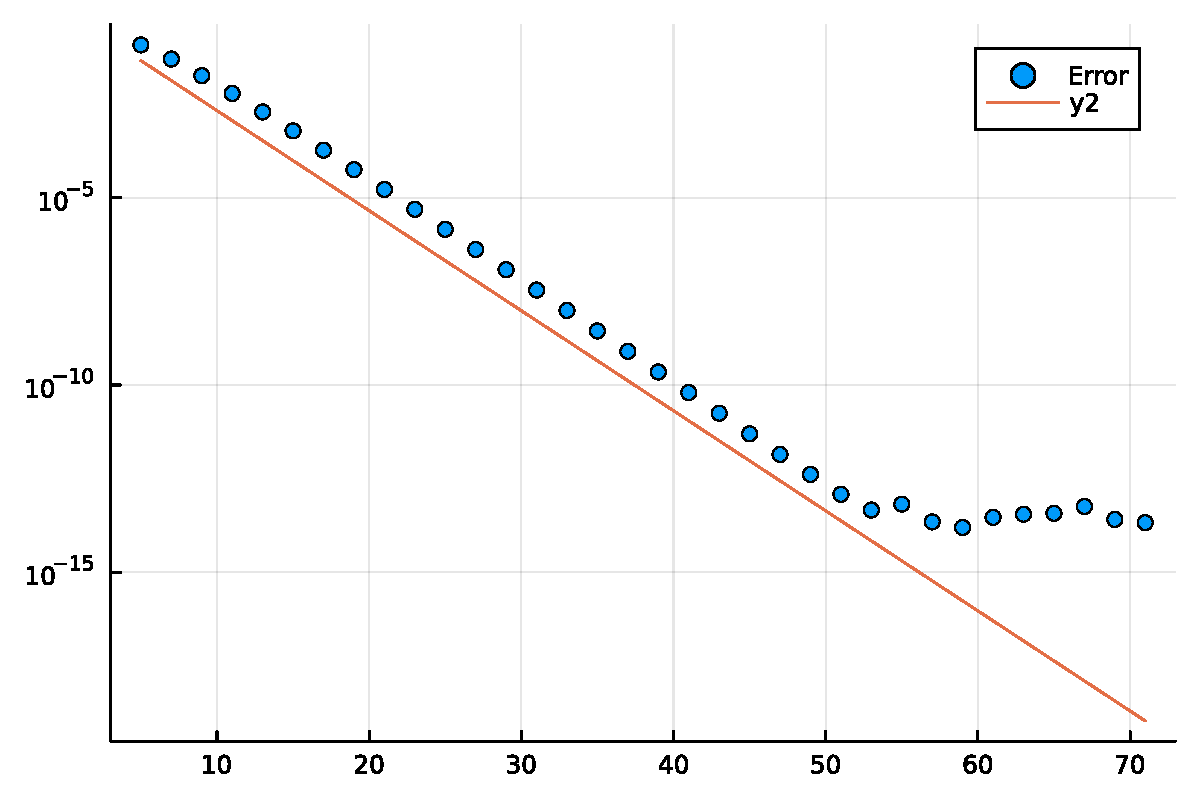
\includegraphics[width=\linewidth]{jl_6X9wr0/Ch1_FD_spectral_periodic_5_1.pdf}

Note that the error decays linearly on a semi-logarithimc plot (or log-linear plot).  This means that the error decays \emph{exponentially fast} with $n$ (we say that the approximation converges exponentially fast).  That is, the error decays as $\mathcal{O}(c^{-n})$ for $n \to \infty$ with $c > 1$.  Recall that the error of the second-order central difference formula decayed as $\mathcal{O}(n^{-2})$.  This type of converge is  called algebraic convergence.  Note how much faster exponential convergence is compared to algebraic convergence.

To derive finite difference approximations to the derivative, we used low degree polynomials to approximate $f'$ locally.  The idea behind \emph{spectral methods} for differential equations (including PDEs) is to use high degree polynomials (or high accuracy interpolants) to approximate solutions to differential equations.

\subsection{Exercises}
\begin{itemize}
\item[1. ] \textbf{(Second-order central difference approximation to the second derivative)} Show that if $f \in C^{4}[x_{j-1}, x_{j+1}]$, then

\end{itemize}
\[
f''(x_j) = \frac{f(x_{j+1}) -  2f(x_{j}) + f(x_{j-1})}{h^2} + \mathcal{O}(h^2), \qquad h \to 0.
\]
\begin{itemize}
\item[2. ] Run the Julia code in this chapter and / or the Matlab code for this chapter (see the Blackboard page of this module) on your own machine.  To run the Julia code, see the document titled Julia on Blackboard.  To run the Matlab code, you'll need to use Chebfun (see the instructions for how to do this \href{https://www.chebfun.org/download/}{here}). 


\item[3. ] Construct, by hand, a polynomial that interpolates $f(x) = {\rm e}^{x}$ at $x = 0, 1, 2$.


\item[4. ] One-sided FD formula?


\item[5. ] Numerical experiment with the fourth order central difference formula?

\end{itemize}


\end{document}
